\begin{SCn}
	
\scnsectionheader{\currentname}
	
\scnstartsubstruct

\scnrelfromlist{дочерний раздел}{Предметная область и онтологий интерфейсных действий пользователей ostis-систем;Предметная область и онтология естественных языков}

\scnheader{Предметная область интерфейсов ostis-систем}
\scniselement{предметная область}
\scnsdmainclasssingle{пользовательский интефейс}
\scnsdclass{командный пользовательский интерфейс;графический пользовательский интерфейс;WIMP-интерфейс;SILK-интерфейс;естественно-языковой интерфейс;речевой интерфейс;пользовательский интерфейс ostis-системы;компонент пользовательского интерфейса;атомарный компонент пользовательского интерфейса;неатомарный компонент пользовательского интерфейса;визуальная часть пользовательского интерфейса ostis-системы;компонент пользовательского интерфейса для представления;компонент вывода;компонент выполнения;параграф;декоративный компонент пользовательского интерфейса;контейнер;меню;строка меню;панель инструментов;панель вкладок;окно;модальное окно;немодальное окно;интерактивный компонент пользовательского интерфейса;флаговая кнопка;радиокнопка;переключатель;кнопка-счетчик;полоса прокрутки;кнопка}


\scnheader{пользовательский интерфейс}
\scnsuperset{командный пользовательский интерфейс}
\scnsuperset{графический пользовательский интерфейс}
\scnaddlevel{1}
\scnsuperset{WIMP-интерфейс}
\scnaddlevel{1}
\scnsuperset{пользовательский интерфейс ostis-системы}
\scnaddlevel{1}
\scnhaselement{Пользовательский интерфейс Метасистемы IMS.ostis}
\scnhaselement{Пользовательский интерфейс ИСС по геометрии}
\scnaddlevel{1}
\scnidtf{Пользовательский интерфейс интеллектуальной справочной системы по геометрии}
\scnaddlevel{-1}
\scnhaselement{Пользовательский интерфейс ИСС по дискретной математике}
\scnaddlevel{1}
\scnidtf{Пользовательский интерфейс интеллектуальной справочной системы по дискретной математике}
\scnaddlevel{-1}
\scnhaselement{Пользовательский интерфейс ИСС по географии}
\scnaddlevel{1}
\scnidtf{Пользовательский интерфейс интеллектуальной справочной системы по географии}
\scnaddlevel{-1}
\scnhaselement{Пользовательский интерфейс ИСС по искусственным нейронным сетям}
\scnaddlevel{1}
\scnidtf{Пользовательский интерфейс интеллектуальной справочной системы по искусственным нейронным сетям}
\scnaddlevel{-1}
\scnhaselement{Пользовательский интерфейс ИСС по лингвистике}
\scnaddlevel{1}
\scnidtf{Пользовательский интерфейс интеллектуальной справочной системы по лингвистике}
\scnaddlevel{-3}
\scnsuperset{SILK-интерфейс}
\scnaddlevel{1}
\scnidtf{(Speech – речь, Image – образ, Language – язык, Knowledge – знание)}
\scnsuperset{естественно-языковой интерфейс}
\scnaddlevel{1}
\scnsuperset{речевой интерфейс}
\scnaddlevel{-2}

\scnheader{пользовательский интерфейс}
\scnexplanation{\textit{пользовательский интерфейс} -- один из наиболее важных компонентов компьютерной системы. Представляет собой совокупность аппаратных и программных средств, обеспечивающих обмен информацией между пользователем и компьютерной системой.}

\scnheader{командный пользовательский интерфейс}
\scnexplanation{\textit{командный пользовательский интерфейс} -- пользовательский интерфейс, при котором обмен информацией между компьютерной системой и пользователем осуществляется путем написания текстовых инструкций или команд.}

\scnheader{графический пользовательский интерфейс}
\scnexplanation{\textit{графический пользовательский интерфейс} -- пользовательский интерфейс, при котором обмен информацией между компьютерной системой и пользователем осуществляется при помощи графических компонентов компьютерной системы.}

\scnheader{WIMP-интерфейс}
\scnexplanation{\textit{WIMP-интерфейс} -- пользовательский интерфейс, при котором обмен информацией между компьютерной системой и пользователем осуществляется в форме диалога при помощью окон, меню и других элементов управления.}

\scnheader{SILK-интерфейс}
\scnexplanation{\textit{SILK-интерфейс} -- пользовательский интерфейс, наиболее приближенный к естественной для человека форме общения. Компьютерная система находит для себя команды, анализируя человеческую речь и находя в ней ключевые фразы. Результат выполнения команд преобразуется в понятную человеку форму, например, в естественно-языковую форму или изображение.}

\scnheader{естественно-языковой интерфейс}
\scnexplanation{\textit{естественно-языковой интерфейс} -- SILK-интерфейс, обмен информацией между компьютерной системой и пользователем в котором происходит за счёт диалога. Диалог ведётся на одном из естественных языков.}

\scnheader{речевой интерфейс}
\scnexplanation{\textit{речевой интерфейс} -- SILK-интерфейс, обмен информацией в котором происходит за счёт диалога, в процессе которого компьютерная система и пользователь общаются с помощью речи. Данный вид интерфейса наиболее приближен к естественному общению между людьми.}

\scnheader{пользовательский интерфейс ostis-системы}
\scnsubset{ostis-система}
\scnexplanation{\textit{пользовательский интерфейс ostis-системы} представляет собой специализированную \textit{ostis-систему}, ориентированную на решение интерфейсных задач, и имеющую в своем составе базу знаний и решатель задач пользовательского интерфейса ostis-системы.\\
Для решения задачи построения пользовательского интерфейса в базе знаний \textit{пользовательского интерфейса ostis-системы} необходимо наличие sc-модели \textit{компонентов пользовательского интерфейса}, \textit{интерфейсных действий пользователей}, а также классификации \textit{пользовательских интерфейсов} вцелом. При проектировании интерфейса используется компонентный подход,который предполагает представление всего интерфейса приложения в виде отдельных специфицированных компонентов, которые могут разрабатываться и совершенствоваться независимо.}

\scnheader{компонент пользовательского интерфейса}
\scnexplanation{\textit{компонент пользовательского интерфейса} -- знак фрагмента базы знаний, имеющий определённую форму внешнего представления на экране.}
\scnsubdividing{атомарный компонент пользовательского интерфейса;неатомарный компонент пользовательского интерфейса}

\scnheader{атомарный компонент пользовательского интерфейса}
\scnexplanation{\textit{атомарный компонент пользовательского интерфейса} -- компонент пользовательского интерфейса, не содержащий в своём составе других компонентов пользовательского интерфейса.}

\scnheader{неатомарный компонент пользовательского интерфейса}
\scnexplanation{\textit{неатомарный компонент пользовательского интерфейса} -- компонент пользовательского интерфейса, состоящий из других компонентов пользовательского интерфейса.}

\scnheader{визуальная часть пользовательского интерфейса ostis-системы}
\scnsubset{неатомарный компонент пользовательского интерфейса}
\scnexplanation{\textit{визуальная часть пользовательского интерфейса ostis-системы} -- часть базы знаний пользовательского интерфейса ostis-системы, содержащая необходимые для отображения пользовательского интерфейса компоненты.}
	
\scnheader{компонент пользовательского интерфейса}
\scnidtf{user interface component}
\scnsuperset{компонент пользовательского интерфейса для отображения}
\scnaddlevel{1}
\scnidtf{presentation user interface component}
\scnaddlevel{-1}
\scnaddlevel{1}
	\scnsuperset{компонент вывода}
	\scnaddlevel{1}
	\scnidtf{output}
	\scnaddlevel{-1}
	\scnaddlevel{1}
		\scnsuperset{компонент вывода изображения}
		\scnaddlevel{1}
		\scnidtf{image-output}
		\scnaddlevel{-1}
		\scnsuperset{компонент вывода графической информации}
		\scnaddlevel{1}
		\scnidtf{graphical-output}
		\scnaddlevel{-1}
			\scnaddlevel{1}
			\scnsuperset{диаграмма}
			\scnaddlevel{1}
			\scnidtf{chart}
			\scnaddlevel{-1}
			\scnsuperset{карта}
			\scnaddlevel{1}
			\scnidtf{map}
			\scnaddlevel{-1}
			\scnsuperset{индикатор выполнения} 
			\scnaddlevel{1}
			\scnidtf{progress-bar}
			\scnaddlevel{-1}
			\scnaddlevel{-1}
		\scnsuperset{компонент вывода видео}
		\scnaddlevel{1}
		\scnidtf{video-output}
		\scnaddlevel{-1}
		\scnsuperset{компонент вывода звука}
		\scnaddlevel{1}
		\scnidtf{sound-output}
		\scnaddlevel{-1}
		\scnsuperset{компонент вывода текста}
		\scnaddlevel{1}
		\scnidtf{text-output}
		\scnaddlevel{-1}
			\scnaddlevel{1}
			\scnsuperset{заголовок}
			\scnaddlevel{1}
			\scnidtf{headline}
			\scnaddlevel{-1}
			\scnsuperset{параграф}
			\scnaddlevel{1}
			\scnidtf{paragraph}
			\scnaddlevel{-1}
			\scnsuperset{сообщение}
			\scnaddlevel{1}
			\scnidtf{message}
			\scnaddlevel{-1}
			\scnaddlevel{-2}
\scnsuperset{декоративный компонент пользовательского интерфейса}
\scnaddlevel{1}
\scnidtf{decorative user interface component}
\scnaddlevel{-1}
	\scnaddlevel{1}
	\scnsuperset{разделитель}
	\scnaddlevel{1}
	\scnidtf{separator}
	\scnaddlevel{-1}
	\scnsuperset{пустое пространство}
	\scnaddlevel{1}
	\scnidtf{blank-space}
	\scnaddlevel{-2}
\scnsuperset{контейнер}
	\scnaddlevel{1}
		\scnidtf{container}
		\scnsuperset{меню}
		\scnaddlevel{1}
		\scnidtf{menu}
		\scnaddlevel{-1}
		\scnsuperset{строка меню}
		\scnaddlevel{1}
		\scnidtf{menu-bar}
		\scnaddlevel{-1}
		\scnsuperset{панель инструментов}
		\scnaddlevel{1}
		\scnidtf{tool-bar}
		\scnaddlevel{-1}
		\scnsuperset{строка состояния}
		\scnaddlevel{1}
		\scnidtf{status-bar}
		\scnaddlevel{-1}
		\scnsuperset{таблично-строковый контейнер}
		\scnaddlevel{1}
		\scnidtf{table-row-container}
		\scnaddlevel{-1}
		\scnsuperset{списковый контейнер}
		\scnaddlevel{1}
		\scnidtf{list-container}
		\scnaddlevel{-1}
		\scnsuperset{таблично-клеточный контейнер}
		\scnaddlevel{1}
		\scnidtf{table-cell-container}
		\scnaddlevel{-1}
		\scnsuperset{древовидный контейнер}
		\scnaddlevel{1}
		\scnidtf{tree-container}
		\scnaddlevel{-1}
		\scnsuperset{панель вкладок}
		\scnaddlevel{1}
		\scnidtf{tab-pane}
		\scnaddlevel{-1}
		\scnsuperset{панель вращения}
		\scnaddlevel{1}
		\scnidtf{spin-pane}
		\scnaddlevel{-1}
		\scnsuperset{узловой контейнер}
		\scnaddlevel{1}
		\scnidtf{tree-node-container}
		\scnaddlevel{-1}
		\scnsuperset{панель прокрутки}
		\scnaddlevel{1}
		\scnidtf{scroll-pane}
		\scnaddlevel{-1}
		\scnsuperset{окно}
		\scnaddlevel{1}
		\scnidtf{window}
		\scnaddlevel{-1}
			\scnaddlevel{1}
			\scnsuperset{модальное окно}
			\scnaddlevel{1}
			\scnidtf{modal-window}
			\scnaddlevel{-1}
			\scnsuperset{немодальное окно}
			\scnaddlevel{1}
			\scnidtf{non-modal-window}
			\scnaddlevel{-4}		
\scnsuperset{интерактивный компонент пользовательского интерфейса}
\scnaddlevel{1}
\scnidtf{interactive user interface component}
\scnaddlevel{-1}
	\scnaddlevel{1}
	\scnsuperset{компонент ввода данных}
	\scnaddlevel{1}
	\scnidtf{data-input-component}
	\scnaddlevel{-1}
		\scnaddlevel{1}
		\scnsuperset{компонент ввода данных с прямой ответной реакцией}
		\scnaddlevel{1}
		\scnidtf{data-input-component-with-direct-feedback}
		\scnaddlevel{-1}
			\scnaddlevel{1}
			\scnsuperset{компонент ввода текста с прямой ответной реакцией}
			\scnaddlevel{1}
			\scnidtf{text-input-component-with-direct-feedback}
			\scnaddlevel{-1}
				\scnaddlevel{1}
				\scnsuperset{многострочное текстовое поле}
				\scnaddlevel{1}
				\scnidtf{multi-line-text-field}
				\scnaddlevel{-1}
				\scnsuperset{однострочное текстовое поле}
				\scnaddlevel{1}
				\scnidtf{single-line-text-field}
				\scnaddlevel{-1}
				\scnaddlevel{-1}
			\scnsuperset{ползунок}
			\scnaddlevel{1}
			\scnidtf{slider}
			\scnaddlevel{-1}
			\scnsuperset{область рисования}
			\scnaddlevel{1}
			\scnidtf{drawing-area}
			\scnaddlevel{-1}
			\scnsuperset{компонент выбора}
			\scnaddlevel{1}
			\scnidtf{selection-component}
			\scnaddlevel{-1}
				\scnaddlevel{1}
				\scnsuperset{компонент выбора нескольких значений}
				\scnaddlevel{1}
				\scnidtf{selection-component-multiple-values}
				\scnaddlevel{-1}
				\scnsuperset{компонент выбора одного значения}
				\scnaddlevel{1}
				\scnidtf{selection-component-single-values}
				\scnaddlevel{-1}
				\scnaddlevel{-1}
			\scnsuperset{компонент выбора данных}
			\scnaddlevel{1}
			\scnidtf{selectable-data-representation}
			\scnaddlevel{-1}	
				\scnaddlevel{1}
				\scnsuperset{флаговая кнопка}
				\scnaddlevel{1}
				\scnidtf{check-box}
				\scnaddlevel{-1}
				\scnsuperset{радиокнопка}
				\scnaddlevel{1}
				\scnidtf{radio-button}
				\scnaddlevel{-1}
				\scnsuperset{переключатель}
				\scnaddlevel{1}
				\scnidtf{toggle-button}
				\scnaddlevel{-1}
				\scnsuperset{выбираемый элемент}
				\scnidtf{selectable-item}
				\scnaddlevel{-2}
		\scnsuperset{компонент ввода данных без прямой ответной реакции}
		\scnaddlevel{1}
		\scnidtf{data-input-component-without-direct-feedback}
		\scnaddlevel{-1}
			\scnaddlevel{1}
			\scnsuperset{кнопка-счётчик}
			\scnaddlevel{1}
			\scnidtf{spin-button}
			\scnaddlevel{-1}
			\scnsuperset{компонент речевого ввода}
			\scnaddlevel{1}
			\scnidtf{speech-input}
			\scnaddlevel{-1}
			\scnsuperset{компонент ввода движений}
			\scnaddlevel{1}
			\scnidtf{motion-input}
			\scnaddlevel{-1}
			\scnaddlevel{-2}
	\scnsuperset{компонент для представления и взаимодействия с пользователем}
	\scnaddlevel{1}
	\scnidtf{presentation-manipulation-component}
	\scnaddlevel{-1}
		\scnaddlevel{1}
		\scnsuperset{активирующий компонент}
		\scnaddlevel{1}
		\scnidtf{activating-component}
		\scnaddlevel{-1}
		\scnsuperset{компонент непрерывной манипуляции}
		\scnaddlevel{1}
		\scnidtf{continuous-manipulation-component}
		\scnaddlevel{-1}
			\scnaddlevel{1}
			\scnsuperset{полоса прокрутки}
			\scnaddlevel{1}
			\scnidtf{scrollbar}
			\scnaddlevel{-1}
			\scnsuperset{компонент редактирования размера}
			\scnaddlevel{1}
			\scnidtf{resizer}
			\scnaddlevel{-1}
			\scnaddlevel{-2}
	\scnsuperset{компонент запроса действий}
	\scnaddlevel{1}
	\scnidtf{operation-trigger-component}
	\scnaddlevel{-1}
		\scnaddlevel{1}
		\scnsuperset{компонент выбора команд}
		\scnaddlevel{1}
		\scnidtf{command-selection-component}
		\scnaddlevel{-1}
			\scnaddlevel{1}
			\scnsuperset{кнопка}
			\scnaddlevel{1}
			\scnidtf{button}
			\scnaddlevel{-1}
			\scnsuperset{пункт меню}
			\scnaddlevel{1}
			\scnidtf{menu-item}
			\scnaddlevel{-1}
			\scnaddlevel{-1}
		\scnsuperset{компонент ввода команд}
		\scnaddlevel{1}
		\scnidtf{command-input-component}
		\scnaddlevel{-1}
		\scnaddlevel{-2}

\scnheader{компонент пользовательского интерфейса для представления}
\scnexplanation{\textit{компонент пользовательского интерфейса для представления} -- компонент пользовательского интерфейса, не подразумевающий взаимодействия с пользователем.}

\scnheader{компонент вывода}
\scnexplanation{\textit{компонент вывода} -- компонент пользовательского интерфейса, предназначенный для представления информации.}

\scnheader{индикатор выполнения}
\scnexplanation{\textit{индикатор выполнения} -- компонент пользовательского интерфейса, предназначенный для отображения процента выполнения какой-либо задачи.}

\scnheader{параграф}
\scnexplanation{\textit{параграф} -- компонент пользовательского интерфейса, предназначенный для отображения блоков текста. Он отделяется от других блоков пустой строкой или первой строкой с отступом.}

\scnheader{декоративный компонент пользовательского интерфейса}
\scnexplanation{\textit{декоративный компонент пользовательского интерфейса} -- компонент пользовательского интерфейса, предназначенный для стилизации интерфейса.}

\scnheader{контейнер}
\scnexplanation{\textit{контейнер} -- компонент пользовательского интерфейса, задача которого состоит в размещении набора компонентов, включённых в его состав.
}

\scnheader{меню}
\scnexplanation{\textit{меню} -- компонент пользовательского интерфейса, содержащий несколько вариантов для выбора пользователем.}

\scnheader{строка меню}
\scnexplanation{\textit{строка меню} -- горизонтальная полоса , содержащая ярлыки меню. Строка меню предоставляет пользователю место в окне, где можно найти большинство основных функций программы.}

\scnheader{панель инструментов}
\scnexplanation{\textit{панель инструментов} -- компонент пользовательского интерфейса, на котором размещаются элементы ввода или вывода данных.}

\scnheader{панель вкладок}
\scnexplanation{\textit{панель вкладок} -- контейнер, который может содержать несколько вкладок (секций) внутри, которые могут быть отображены, нажав на вкладке с названием в верхней части панели. Одновременно отображается только одна вкладка.}

\scnheader{окно}
\scnexplanation{\textit{окно} -- обособленная область экрана, содержащая различные элементы пользовательского интерфейса. Окна могут располагаться поверх друг друга.}

\scnheader{модальное окно}
\scnexplanation{\textit{модальное окно} -- окно, которое блокирует работу пользователя с системой до тех пор, пока пользователь окно не закроет.}

\scnheader{немодальное окно}
\scnexplanation{\textit{немодальное окно} -- окно, которое позволяет выполнять переключение между данным окном и другим окном без необходимости закрытия окна.}

\scnheader{интерактивный компонент пользовательского интерфейса}
\scnexplanation{\textit{интерактивный компонент пользовательского интерфейса} -- компонент пользовательского интерфейса, с помощью которого осуществляется взаимодействие с пользователем.}

\scnheader{флаговая кнопка}
\scnexplanation{\textit{флаговая кнопка} -- компонент пользовательского интерфейса, позволяющий пользователю управлять параметром с двумя состояниями — включено и отключено.}

\scnheader{радиокнопка}
\scnexplanation{\textit{радиокнопка} -- компонент пользовательского интерфейса, который позволяет пользователю выбрать одну опцию из предопределенного набора.}

\scnheader{переключатель}
\scnexplanation{\textit{переключатель} -- компонент пользовательского интерфейса, который позволяет пользователю переключаться между двумя состояниями.}

\scnheader{кнопка-счетчик}
\scnexplanation{\textit{кнопка-счетчик} -- компонент пользовательского интерфейса, как правило, ориентированный вертикально, с помощью которого пользователь может изменить значение в прилегающем текстовом поле, в результате чего значение в текстовом поле увеличивается или уменьшается.}


\scnheader{полоса прокрутки}
\scnexplanation{\textit{полоса прокрутки} -- компонент пользовательского интерфейса, который используется для отображения компонентов пользовательского интерфейса, больших по размеру, чем используемый для их отображения контейнер.}

\scnheader{кнопка}
\scnexplanation{\textit{кнопка} -- компонент пользовательского интерфейса, при нажатии на который происходит программно связанное с этим нажатием действие либо событие.}

\scnheader{Стартовая страница пользовательского интерфейса Метасистемы IMS.ostis}
\scniselement{Визуальная часть пользовательского интерфейса Метасистемы IMS.ostis}
	\scnaddlevel{1}
	\scnsubset{визуальная часть пользовательского интерфейса ostis-системы}
	\scnrelto{часть}{Пользовательский интерфейс Метасистемы IMS.ostis}
	\scnaddlevel{-1}
\scniselement{окно}
\scnrelfrom{иллюстрация}{
\scnfileimage{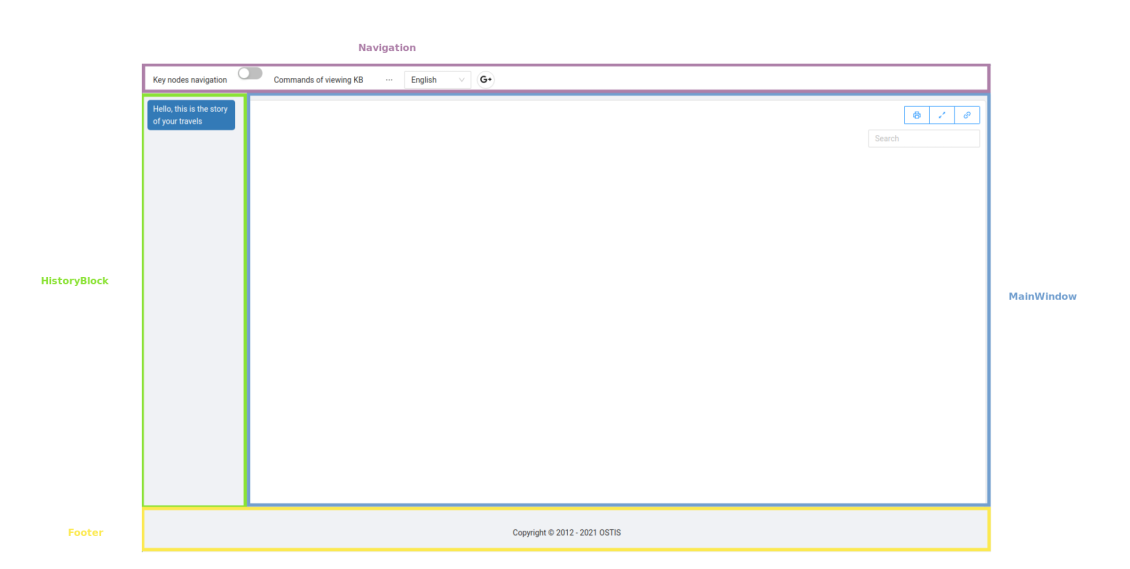
\includegraphics[width=1\linewidth]{figures/sd_ui/startPage.png}}}
\scnaddlevel{1}
\scnaddlevel{-1}
\scnrelfromset{декомпозиция}{
Панель навигации\\
	\scnaddlevel{1}
	\scniselement{неатомарный компонент пользовательского интерфейса}
	\scnrelfromset{декомпозиция}{
	Главное меню\\	
		\scnaddlevel{1}
		\scniselement{меню}
		\scnrelfromset{декомпозиция}{
		Пункт меню для навигации по ключевым понятиям\\
			\scnaddlevel{1}
			\scniselement{пункт меню}
			\scnaddlevel{-1}
		;Пункт меню для выполнения команд просмотра базы знаний\\
			\scnaddlevel{1}
			\scniselement{пункт меню}
			\scnaddlevel{-1}			
		;Компонент перехода в экспертный режим\\
			\scnaddlevel{1}
			\scniselement{переключатель}
			\scnaddlevel{-1}
	}
	\scnaddlevel{-1}
	;Компонент выбора языка\\
		\scnaddlevel{1}
		\scniselement{компонент выбора одного значения}
		\scnaddlevel{-1}
	;Компонент авторизации\\
		\scnaddlevel{1}
		\scniselement{кнопка}
		\scnaddlevel{-1}}
	\scnaddlevel{-1}
;Блок истории запросов пользователя\\
	\scnaddlevel{1}
	\scniselement{неатомарный компонент пользовательского интерфейса}
	\scnaddlevel{-1}
;Основной блок\\
	\scnaddlevel{1}
	\scniselement{неатомарный компонент пользовательского интерфейса}
	\scnrelfromset{декомпозиция}{
	Главное окно\\
		\scnaddlevel{1}
		\scniselement{окно}
		\scnaddlevel{-1}
	;Панель инструментов\\
		\scnaddlevel{1}
		\scniselement{неатомарный компонент пользовательского интерфейса}
		\scnrelfromset{декомпозиция}{Кнопка отправки содержимого главного окна на печать\\
			\scnaddlevel{1}
			\scniselement{кнопка}
			\scnaddlevel{-1}
		;Кнопка управления видимостью блока истории запросов пользователя\\
			\scnaddlevel{1}
			\scniselement{кнопка}
			\scnaddlevel{-1}
		;Кнопка отображения ссылки на текущий запрос пользователя\\
			\scnaddlevel{1}
			\scniselement{кнопка}
			\scnaddlevel{-1}
		;Поле поиска\\	
			\scnaddlevel{1}
			\scniselement{однострочное текстовое поле}
			\scnaddlevel{-1}
		}
	\scnaddlevel{-1}
	}
\scnaddlevel{-1}
;Панель отображения информации об авторских правах\\
	\scnaddlevel{1}
	\scniselement{неатомарный компонент пользовательского интерфейса}
	\scnaddlevel{-1}
}

\bigskip
\scnendstruct \scnendcurrentsectioncomment
\end{SCn}